\section{Sauvegarde}

% À charge à Anthony et Rémi de remplir cette partie
% Indications :
%  Reprise sur panne
%  Réseau
%  Stockage
%  Matériel
%  Compatibilité (la solution de stockage doit compatible avec le top 10 des solutions de sauvegarde les plus communes, cf. le CdCF)...
% 
% Bon courage ;-)

\subsection{Problématique}

Il est indiqué dans le cahier des charges que la suite logicielle doit pouvoir synchroniser des données, à la fois entre postes clients et serveur local, mais également entre serveur local et serveur central.
Cette demande pose les problèmes de la disponibilité du serveur local et de l'intégrité des données. Différentes architectures vont être proposées afin de garantir ces contraintes.

\subsection{Cluster}

Une première solution utilisant la technologie du \textit{cluster} peut être envisagée. Cette technique permet de créer un groupe logique de serveurs qui s'exécutent simultanément tout en donnant l'impression aux utilisateurs de ne constituer qu'un seul serveur.
En considérant le matériel existant, et le fait que l'achat de serveur dédié pour ce cluster serait couteux au client, une solution de \textit{clustering} peut être effectuée grâce à de simples postes clients qu'il faut configurer comme des serveurs. Les étapes de cette configuration sera fournie dans le manuel de déploiement.
\
Deux architectures différentes sont proposées :
\begin{itemize}
	\item Deux postes clients ( configurés comme des serveurs maître/esclave) sont reliés directement par un cable eternet, ce qui va permettre de dupliquer au fur et à mesure toutes les données. Le serveur maître transmet les données au serveur esclave, et en cas d'incident sur le serveur maître, c'est le serveur esclave qui reprend la main.
	% Schéma du cluster relié directement
	\item Les deux postes ne sont pas directement reliés, mais c'est le routeur qui va transmettre les données aux deux serveurs. Cette  solution permet d'augmenter la distance entre les deux serveurs, voir d'utiliser des locaux différents en évitant ainsi une coupure d'électricité au niveau des deux locaux, ou bien la propagation d'un incendie. Par contre cette solution, va augmenter de manière significative l'utilisation réseau, ce qui n'est pas négligeable vu les contraintes des communications réseaux.
	% Schéma du cluster avec la passerelle
\end{itemize}

\begin{figure}[htbp]
    \centering
	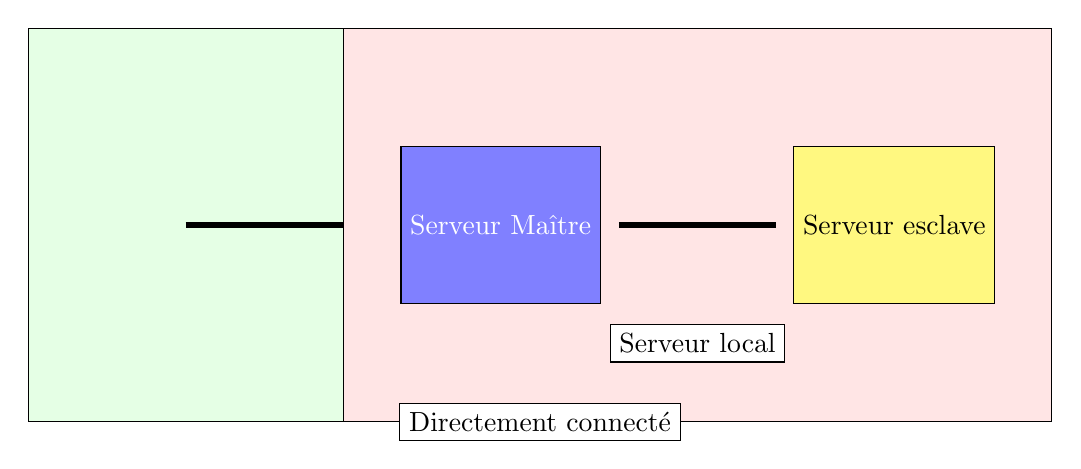
\begin{tikzpicture}
	    % Styles :
		\tikzstyle{titre}=[rectangle,draw,fill=white,text=black]
		\tikzstyle{symbole}=[rectangle,text=black, scale=4]
		\tikzstyle{serveurloc1}=[rectangle,draw,fill=blue!50,text=white, minimum height=2cm]
		\tikzstyle{serveurloc2}=[rectangle,draw,fill=yellow!50,text=black, minimum height=2cm]
		\tikzstyle{serveurcentral}=[rectangle,draw,fill=red!50,text=black, minimum height=2cm]
		
		% #### CADRE VERT :
		% Fond :
		\draw[fill=green!10] (0,6) rectangle (13, 11);
		\draw[fill=red!10] (4,11) rectangle (13, 6);
		% Titres :
		\node[titre] at (6.50,6.00) {Directement connecté};
		\node[titre] at (8.50,7.00) {Serveur local};
		% Serveurs :
		\node[serveurloc1] at (6.00,8.50) {Serveur Maître};
		\node[serveurloc2] at (11.00,8.50) {Serveur esclave};
		% Traits :
		\draw[line width=2pt] (2, 8.5) -- (4, 8.5);
		\draw[line width=2pt] (7.5, 8.5) -- (9.5, 8.5);
		% Utilisateurs :
		\umlactor[x=1.00, y=8.50]{Utilisateur}
	\end{tikzpicture}
	\caption{Cluster}
	\label{explicationcodeco}
\end{figure}

\subsection{Reprise sur panne}
% explication priorités 

\subsection{Sauvegarde en dure}

Une deuxième solution peut être mise en oeuvre de manière complémentaire au \textit{cluster} afin de mieux respecter la contrainte concernant l'intégrité des données. 
